\textbf{Consulta básica}: Encontrar todos los estudiantes de la carrera de \textit{`Ingeniería'}:

\begin{figure}[H]
  \centering
  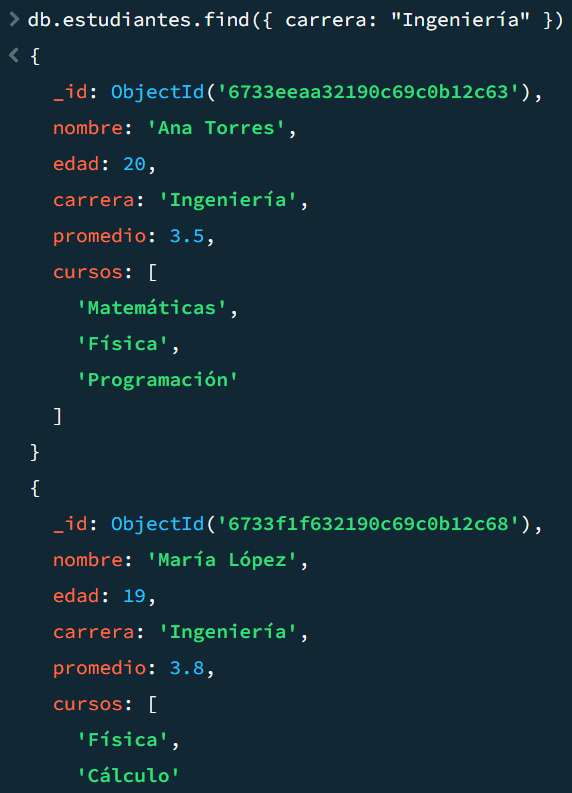
\includegraphics[scale = 0.8]{Imagenes/parte3/3.1.png}
  \caption{Consulta básica}
\end{figure}

\textbf{Operador de comparación \emph{\$gt}}: Obtener estudiantes con un \textit{promedio superior a 3.5}:

\begin{figure}[H]
  \centering
  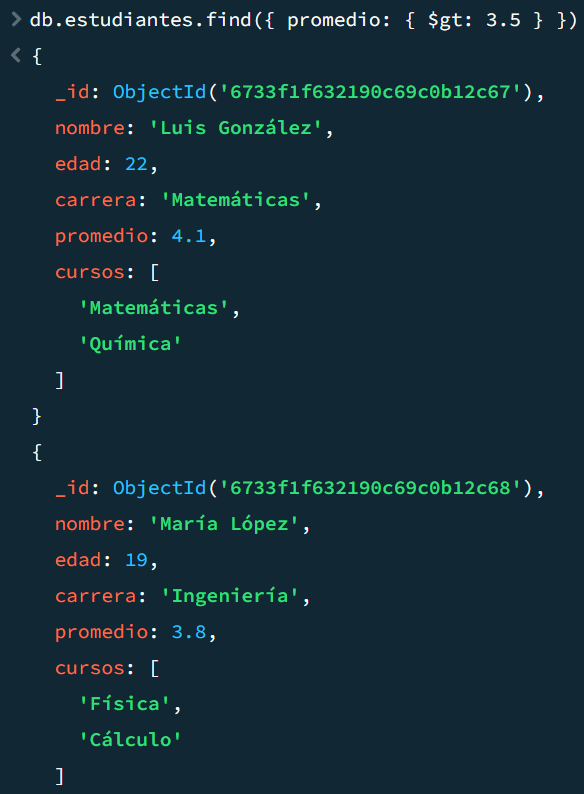
\includegraphics[scale = 0.8]{Imagenes/parte3/3.2.png}
  \caption{Consulta gt}
\end{figure}

\textbf{Operador de comparación \emph{\$lt}}: Buscar estudiantes \textit{menores de 21 años}:

\begin{figure}[H]
  \centering
  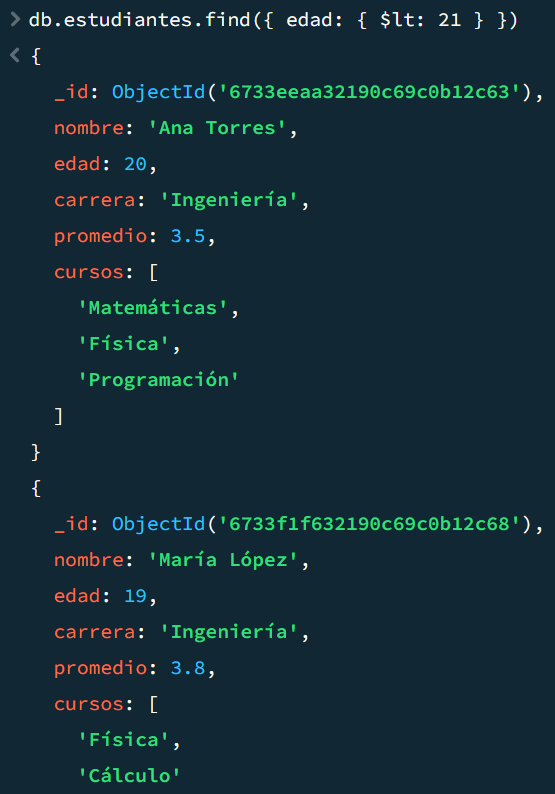
\includegraphics[scale = 0.8]{Imagenes/parte3/3.3.png}
  \caption{Consulta lt}
\end{figure}

\textbf{Operador \emph{\$in}}: Encontrar estudiantes que están \textit{inscritos en el curso de `Matemáticas' o `Física'}:

\begin{figure}[H]
  \centering
  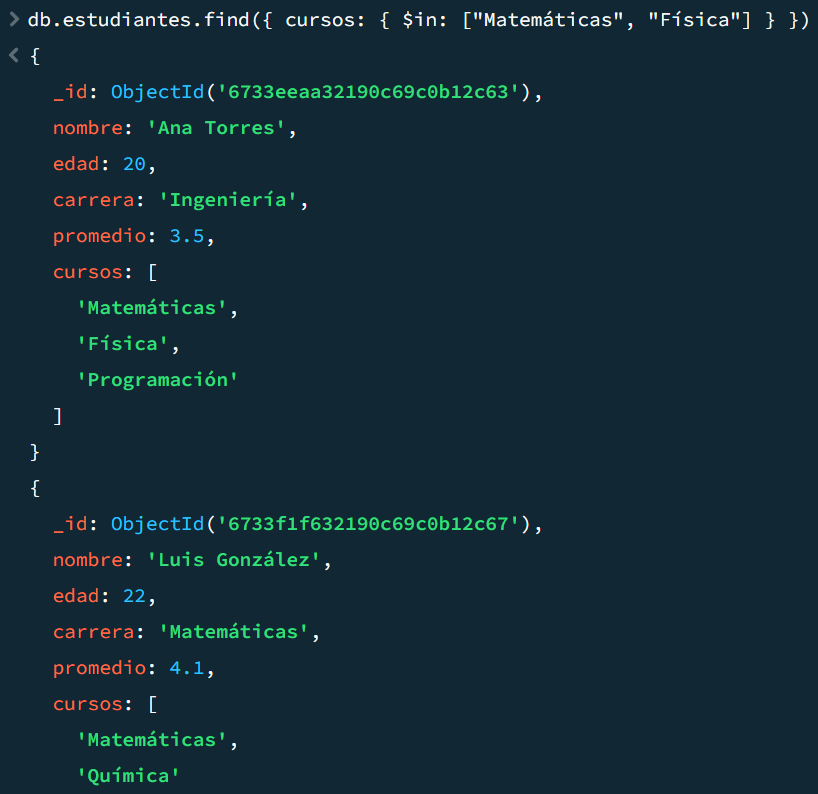
\includegraphics[scale = 0.8]{Imagenes/parte3/3.4.png}
  \caption{Consulta in}
\end{figure}

\textbf{Operador \emph{\$and}}: Obtener estudiantes de la \textit{carrera de `Ingeniería' con un promedio mayor a 3.5}:

\begin{figure}[H]
  \centering
  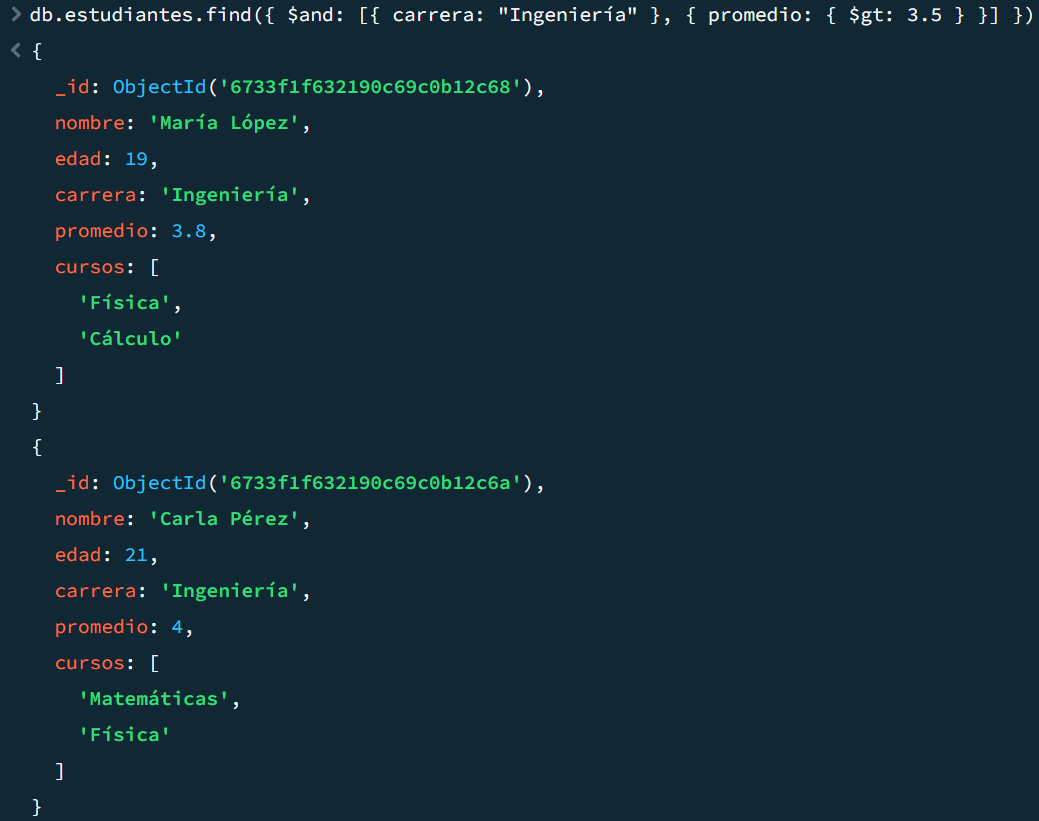
\includegraphics[scale = 0.6]{Imagenes/parte3/3.5.png}
  \caption{Consulta and}
\end{figure}

\textbf{Operador \emph{\$or}}: Obtener estudiantes cuyo \textit{promedio sea mayor a 4.0 o que estén en el curso de `Biología'}:

\begin{figure}[H]
  \centering
  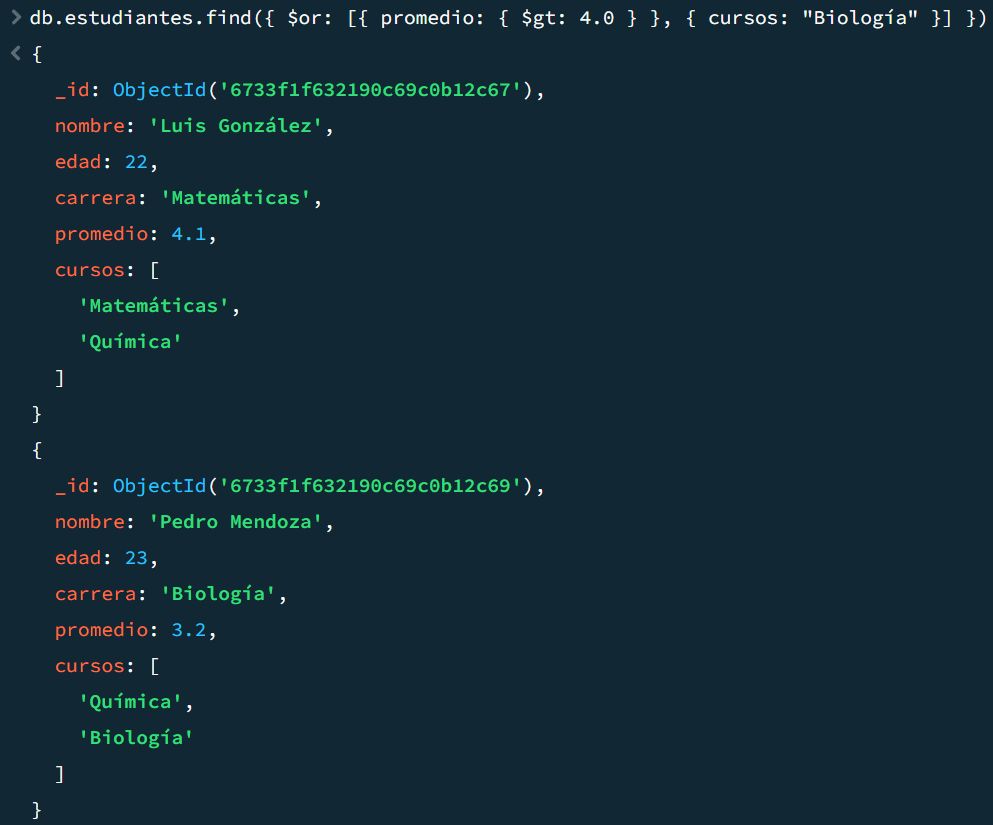
\includegraphics[scale = 0.6]{Imagenes/parte3/3.6.png}
  \caption{Consulta or}
\end{figure}

\textbf{Consulta de proyección}: Mostrar solo los \textit{nombres y promedios} de los estudiantes:

\begin{figure}[H]
  \centering
  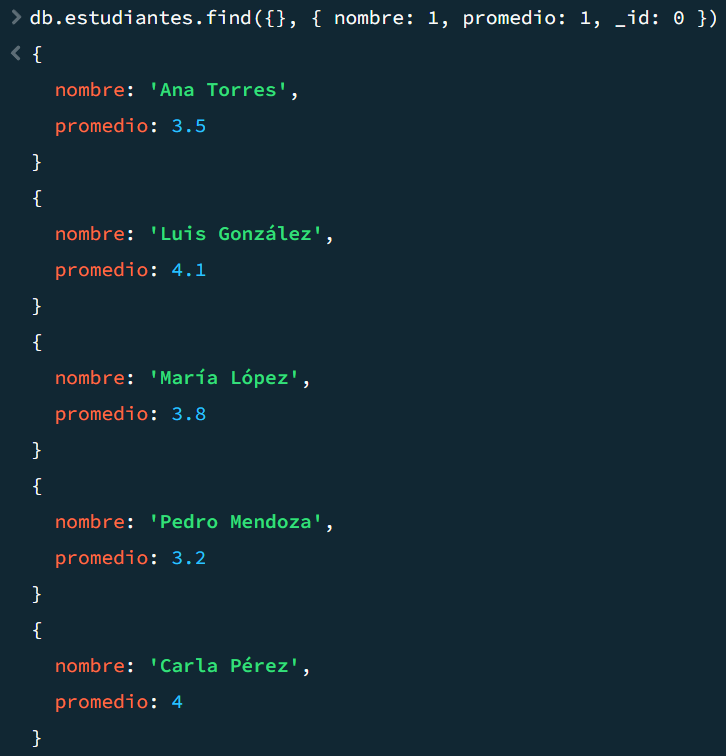
\includegraphics[scale = 0.8]{Imagenes/parte3/3.7.png}
  \caption{Consulta de proyección}
\end{figure}